\section{Experiments}
\label{sec:exp}
\begin{table*}[htb!]
	\begin{center}
		\begin{tabular}{l|l|c|c|c|c|c}
			\hline \bf Corpus &Task& \#Train & \#Dev & \#Test   & \#Label &Metrics\\ \hline \hline
			\multicolumn{6}{@{\hskip1pt}r@{\hskip1pt}}{Single-Sentence Classification (GLUE)} \\ \hline
			CoLA & Acceptability&8.5k & 1k & 1k & 2 & Matthews corr\\ \hline
			SST-2 & Sentiment&67k & 872 & 1.8k & 2 & Accuracy\\ \hline \hline
			\multicolumn{6}{@{\hskip1pt}r@{\hskip1pt}}{Pairwise Text Classification (GLUE)} \\ \hline
			MNLI & NLI& 393k& 20k & 20k& 3 & Accuracy\\ \hline
            RTE & NLI &2.5k & 276 & 3k & 2 & Accuracy \\ \hline
            WNLI & NLI &634& 71& 146& 2 & Accuracy \\ \hline
			QQP & Paraphrase&364k & 40k & 391k& 2 & Accuracy/F1\\ \hline
            MRPC & Paraphrase &3.7k & 408 & 1.7k& 2&Accuracy/F1\\ \hline
			\multicolumn{5}{@{\hskip1pt}r@{\hskip1pt}}{Text Similarity (GLUE)} \\ \hline
			STS-B & Similarity &7k &1.5k& 1.4k &1 & Pearson/Spearman corr\\ \hline

\multicolumn{6}{@{\hskip1pt}r@{\hskip1pt}}{Relevance Ranking (GLUE)} \\ \hline \hline
			QNLI & QA/NLI& 108k &5.7k&5.7k&2& Accuracy\\ \hline \hline
			\multicolumn{6}{@{\hskip1pt}r@{\hskip1pt}}{Pairwise Text Classification} \\ \hline
			SNLI & NLI& 549k &9.8k&9.8k&3& Accuracy\\ \hline
			SciTail & NLI& 23.5k &1.3k&2.1k&2& Accuracy\\ \hline

		\end{tabular}
	\end{center}
%	\lgspace
	\caption{Summary of the three benchmarks: GLUE, SNLI and SciTail.
	}
	\label{tab:datasets}
%\lgspace
\end{table*}

We evaluate the proposed {\MNAME} on three popular NLU benchmarks: GLUE \cite{wang2018glue}, SNLI \cite{snli2015}, and SciTail \cite{scitail}. 
We compare MT-DNN with existing state-of-the-art models including BERT 
and demonstrate the effectiveness of MTL with and without model fine-tuning using GLUE and domain adaptation using both SNLI and SciTail. 

%%%%%%%%%%%%%%%%%%%%%%%%%%%%%%%%%%%%%%%%%
% DATA SETS
%%%%%%%%%%%%%%%%%%%%%%%%%%%%%%%%%%%%%%%%%
%\subsection{Experiment Setup}
%\noindent \textbf{Datasets:} 
\subsection{Datasets}
\label{subsec:dataset}
This section briefly describes the GLUE, SNLI, and SciTail datasets, as summarized in Table~\ref{tab:datasets}.

\paragraph{GLUE} The General Language Understanding Evaluation (GLUE) benchmark is a collection of nine NLU tasks as in Table~\ref{tab:datasets}, including question answering, sentiment analysis, text similarity and textual entailment; it is considered well-designed for evaluating the generalization and robustness of NLU models. 

\paragraph{SNLI}
The Stanford Natural Language Inference (SNLI) dataset contains 570k human annotated sentence pairs, in which the premises are drawn from the captions of the Flickr30 corpus and hypotheses are manually annotated \cite{snli2015}. %The evaluation metric is accuracy as well.
This is the most widely used entailment dataset for NLI.
The dataset is used only for domain adaptation in this study.

\paragraph{SciTail}
This is a textual entailment dataset derived from a science question answering (SciQ) dataset \cite{scitail}. The task involves assessing whether a given premise entails a given hypothesis.  
In contrast to other entailment datasets mentioned previously, the hypotheses in SciTail are created from science questions while the corresponding answer candidates and premises come from relevant web sentences retrieved from a large corpus. As a result, these sentences are linguistically challenging and the lexical similarity of premise and hypothesis is often high, thus making SciTail particularly difficult. 
The dataset is used only for domain adaptation in this study.

\subsection{Implementation details}
\label{subsec:impl}
Our implementation of MT-DNN is based on the PyTorch implementation of BERT\footnote{https://github.com/huggingface/pytorch-pretrained-BERT}.
We used Adamax \cite{kingma2014adam} as our optimizer with a learning rate of 5e-5 and a batch size of 32 by following \citet{bert2018}. 
The maximum number of epochs was set to 5. 
A linear learning rate decay schedule with warm-up over 0.1 was used, unless stated otherwise. %We set the number of steps to 5 with a dropout rate of 0.1.
We also set the dropout rate of all the task specific layers as 0.1, except 0.3 for MNLI and 0.05 for CoLa. 
To avoid the exploding gradient problem, we clipped the gradient norm within 1. 
All the texts were tokenized using wordpieces, and were chopped to spans no longer than 512 tokens.

%%%%%%%%%%%%%%%%%%%%%%%%%%%%%
% Results tables
%%%%%%%%%%%%%%%%%%%%%%%%%%%%%

\begin{table*}[htb!]
\small
	\begin{center}
		\begin{tabular}{l|@{\hskip1pt}l@{\hskip1pt}|@{\hskip1pt}c@{\hskip1pt}|@{\hskip1pt}c@{\hskip1pt}|@{\hskip1pt}c@{\hskip1pt}|@{\hskip1pt}c@{\hskip1pt}|@{\hskip1pt}c|@{\hskip1pt}c|@{\hskip1pt}c |@{\hskip1pt} c |@{\hskip1pt} c|@{\hskip1pt} c}
			\hline \bf Model &CoLA&	SST-2 &MRPC& STS-B&QQP&MNLI-m/mm&QNLI&RTE&WNLI&AX &\textbf{Score}\\ 
			% &MCC &Acc &Acc/F1&P/S Corr&Acc/F1 &Acc &Acc &Acc &Acc &Acc & \\ 
			& 8.5k &67k &3.7k &7k &364k &393k &108k &2.5k &634 & & \\ \hline \hline
			BiLSTM+ELMo+Attn $^1$&36.0 &90.4 &84.9/77.9 &75.1/73.3 &64.8/84.7 &76.4/76.1 &- &56.8 &65.1 &26.5 &70.5 \\ \hline
			\begin{tabular}{@{}c@{}}Singletask Pretrain \\Transformer $^2$   \end{tabular}
			 &45.4 &91.3 &82.3/75.7&82.0/80.0 &70.3/88.5 &82.1/81.4 &- &56.0 &53.4  &29.8 &72.8 \\ \hline
			GPT on STILTs $^3$ &47.2 &93.1 &87.7/83.7 &85.3/84.8 &70.1/88.1 &80.8/80.6 &- &69.1 &65.1 &29.4 &76.9 \\ \hline
			BERT$_{\text{LARGE}}^4$ & 60.5 &94.9 &89.3/85.4 &87.6/86.5 &72.1/89.3 &86.7/85.9 &92.7 &70.1 &65.1	&39.6 & 80.5\\ \hline
%{\MNAME} &\textbf{61.5} &\textbf{95.6} &\color{blue}{\textbf{90.0/86.7}} &\textbf{88.3/87.7} &\color{blue}{\textbf{72.4/89.6}} &\textbf{86.7/86.0}	&98.0 &75.5 &\textbf{65.1}	&40.3 &82.2 \\ \hline
            {\MNAME}\textsubscript{no-fine-tune} & 58.9 &94.6 &\color{blue}{\textbf{90.1/86.4}} &89.5/88.8 &\color{blue}{\textbf{72.7/89.6}} &86.5/85.8	&\color{blue}{\textbf{93.1}} &79.1 &65.1	&39.4 &81.7 \\ \hline \hline
			{\MNAME} & \textbf{62.5} &\textbf{95.6} &\color{blue}{\textbf{91.1/88.2}} &\textbf{89.5/88.8} &\color{blue}{\textbf{72.7/89.6}} &\textbf{86.7/86.0}	&\color{blue}{\textbf{93.1}} &\textbf{81.4} &65.1	&\textbf{40.3} &\textbf{82.7} \\ \hline \hline
			{Human Performance} &66.4&97.8&86.3/80.8    &92.7/92.6	&59.5/80.4	&92.0/92.8	&91.2	&93.6	&95.9 &- & 87.1\\ \hline
		\end{tabular}
	\end{center}
	\caption{GLUE test set results scored using the GLUE evaluation server. The number below each task denotes the number of training examples. The state-of-the-art results are in \textbf{bold}, and the results on par with or pass human performance are in {\color{blue}\textbf{bold}}. MT-DNN uses BERT\textsubscript{LARGE} to initialize its shared layers. 
	All the results are obtained from \href{https://gluebenchmark.com/leaderboard}{https://gluebenchmark.com/leaderboard} on February 25, 2019. 
	% Note that all the results are scored on the latest GLUE test set; the \textit{old} version of GLUE datasets expired on January 30, 2019 and we report its result in the appendix. Please refer to https://gluebenchmark.com for detailed information. 
	Model references: $^1$:\protect\cite{wang2018glue} ; $^2$:\protect\cite{gpt2018}; $^3$: \protect\cite{phang2018sentence}; $^4$:\protect\cite{bert2018}.
	%Note that MT-DNN (v2) denotes results on the latest GLUE test set, and MT-DNN the test results reported on January 15, 2019, on the \textit{old} version of GLUE test set which was expired on January 30, 2019.
	% \JG{Results to be updated by Xiaodong and Pengcheng.}  %\textcolor{red}{TODO: update results of our model.}
	}
	\label{tab:glue_test}
%\lgspace
\end{table*}
\begin{table*}[h!]
	\begin{center}
		\begin{tabular}{l|c@{\hskip1pt}|c@{\hskip1pt}|c@{\hskip1pt}|c@{\hskip1pt}|c@{\hskip1pt}|@{\hskip1pt}c @{\hskip1pt}|c @{\hskip1pt}|c@{\hskip1pt}}
			\hline \bf Model &MNLI-{m/mm} & QQP & RTE & QNLI (v1/v2)  &MRPC & CoLa &SST-2  & STS-B \\ \hline \hline
			BERT$_{\text{LARGE}}$& 86.3/86.2 &91.1/88.0 &71.1 &90.5/92.4 &89.5/85.8 &61.8 &93.5 &89.6/89.3\\
			\hline
			ST-DNN &86.6/86.3 & 91.3/88.4 &  72.0& 96.1/- & 89.7/86.4 &- &- &-\\ \hline
            %{\MNAME}_{wft}  &\textbf{87.1/86.6}& 91.5/88.6& \textbf{83.4} & \textbf{97.3/92.9} & 90.5/87.1& 62.4& 94.1  &90.1/89.5\\ \hline
            {\MNAME}  &\textbf{87.1/86.7} &\textbf{91.9/89.2} &\textbf{83.4}&\textbf{97.4/92.9} &\textbf{91.0/87.5} &\textbf{63.5}& \textbf{94.3}&\textbf{90.7/90.6} \\ \hline

		\end{tabular}
	\end{center}
	\caption{GLUE dev set results. The best result on each task is in \textbf{bold}. 
	% BERT\textsubscript{LARGE} is the large BERT model released by the authors, and is fine-tuned for each single task. 
	The Single-Task DNN (ST-DNN) uses the same model architecture as MT-DNN. But its shared layers are the pre-trainedBERT model without being refined via MTL. We fine-tuned ST-DNN for each GLUE task using task-specific data.
	There have been two versions of the QNLI dataset. V1 is expired on January 30, 2019. The current version is v2.
	% But instead of fine-tuning one model for all tasks using MTL, we create multiple ST-DNNs, one for each task using only in-domain data for fine-tuning. ST-DNNs and 
	MT-DNN use BERT\textsubscript{LARGE} as their initial shared layers. %Note that - denotes the same model structure of BERT\textsubscript{LARGE} and ST-DNN, and thus they produce the same results.
	}
	\label{tab:glue_dev}
\end{table*}

\subsection{GLUE Main Results}
\label{subsec:results}
We compare MT-DNN with its variants and a list of state-of-the-art models that have been submitted to the GLUE leaderboard. The results are shown in Tables \ref{tab:glue_test} and \ref{tab:glue_dev}. 
%It is worth noting that the test results are generated directly from the official GLUE leaderboard server since the test data is not accessible for us.
% is hidden from the leaderboard participants.

\paragraph{BERT\textsubscript{LARGE}} This is the large BERT model released by the authors, which we used as a baseline. We fine-tuned the model for each GLUE task on task-specific data.

\paragraph{MT-DNN} This is the proposed model described in Section 3. We used the pre-trained BERT\textsubscript{LARGE} to initialize its shared layers, refined the model via MTL on all GLUE tasks, and fine-tuned the model for each GLUE task using task-specific data. The test results in Table~\ref{tab:glue_test} show that MT-DNN outperforms all existing systems on all tasks, except WNLI, creating new state-of-the-art results on eight GLUE tasks and pushing the benchmark to 82.7\%, which amounts to 2.2\% absolution improvement over BERT\textsubscript{LARGE}. Since MT-DNN uses BERT\textsubscript{LARGE} to initialize its shared layers, the gain is mainly attributed to the use of MTL in refining the shared layers. 
MTL is particularly useful for the tasks with little in-domain training data. 
As we observe in the table, on the same type of tasks, the improvements over BERT are much more substantial for the tasks with less in-domain training data than those with more in-domain labels, even though they belong to the same task type, e.g., the two NLI tasks: RTE vs. MNLI, and the two paraphrase tasks: MRPC vs. QQP.

\paragraph{MT-DNN\textsubscript{no-fine-tune}} Since the MTL of MT-DNN uses all GLUE tasks, it is possible to directly apply MT-DNN to each GLUE task without fine-tuning.
The results in Table 2 show that MT-DNN\textsubscript{no-fine-tune} still outperforms BERT\textsubscript{LARGE} consistently among all tasks but CoLA. Our analysis shows that CoLA is a challenge task with much smaller in-domain data than other tasks, and its task definition and dataset are unique among all GLUE tasks, making it difficult to benefit from the knowledge learned from other tasks. As a result, MTL tends to underfit the CoLA dataset. In such a case, fine-tuning is necessary to boost the performance. As shown in Table~\ref{tab:glue_test}, the accuracy improves from 58.9\% to 62.5\% after fine-tuning, even though only a very small amount of in-domain data is available for adaptation. This, together with the fact that the fine-tuned MT-DNN significantly outperforms the fine-tuned BERT\textsubscript{LARGE} on CoLA (62.5\% vs. 60.5\%), reveals that the learned MT-DNN representation allows much more effective domain adaptation than the pre-trained BERT representation. We will revisit this topic with more experiments in Section~\ref{subsec:domain}.

The gain of MT-DNN is also attributed to its flexible modeling framework which allows us to incorporate the task-specific model structures and training methods which have been developed in the single-task setting, effectively leveraging the existing body of research. Two such examples are the use of the SAN answer module for the pairwise text classification output module and the pairwise ranking loss for the QNLI task which by design is a binary classification problem in GLUE. To investigate the relative contributions of these modeling design choices, we implement a variant of MT-DNN as described below.

\paragraph{ST-DNN} ST-DNN stands for Single-Task DNN. It uses the same model architecture as MT-DNN. But its shared layers are the pre-trained BERT model without being refined via MTL. We then fine-tuned ST-DNN for each GLUE task using task-specific data. Thus, for pairwise text classification tasks, the only difference between their ST-DNNs and BERT models is the design of the task-specific output module. The results in Table~\ref{tab:glue_dev} show that on all four tasks (MNLI, QQP, RTE and MRPC) ST-DNN outperforms BERT, justifying the effectiveness of the SAN answer module. We also compare the results of ST-DNN and BERT on QNLI. While ST-DNN is fine-tuned using the pairwise ranking loss, BERT views QNLI as binary classification and is fine-tuned using the cross entropy loss. ST-DNN significantly outperforms BERT demonstrates clearly the importance of problem formulation.


\subsection{Domain Adaptation Results on SNLI and SciTail}
\label{subsec:domain}

\begin{figure}[h!]
    \centering
 {
	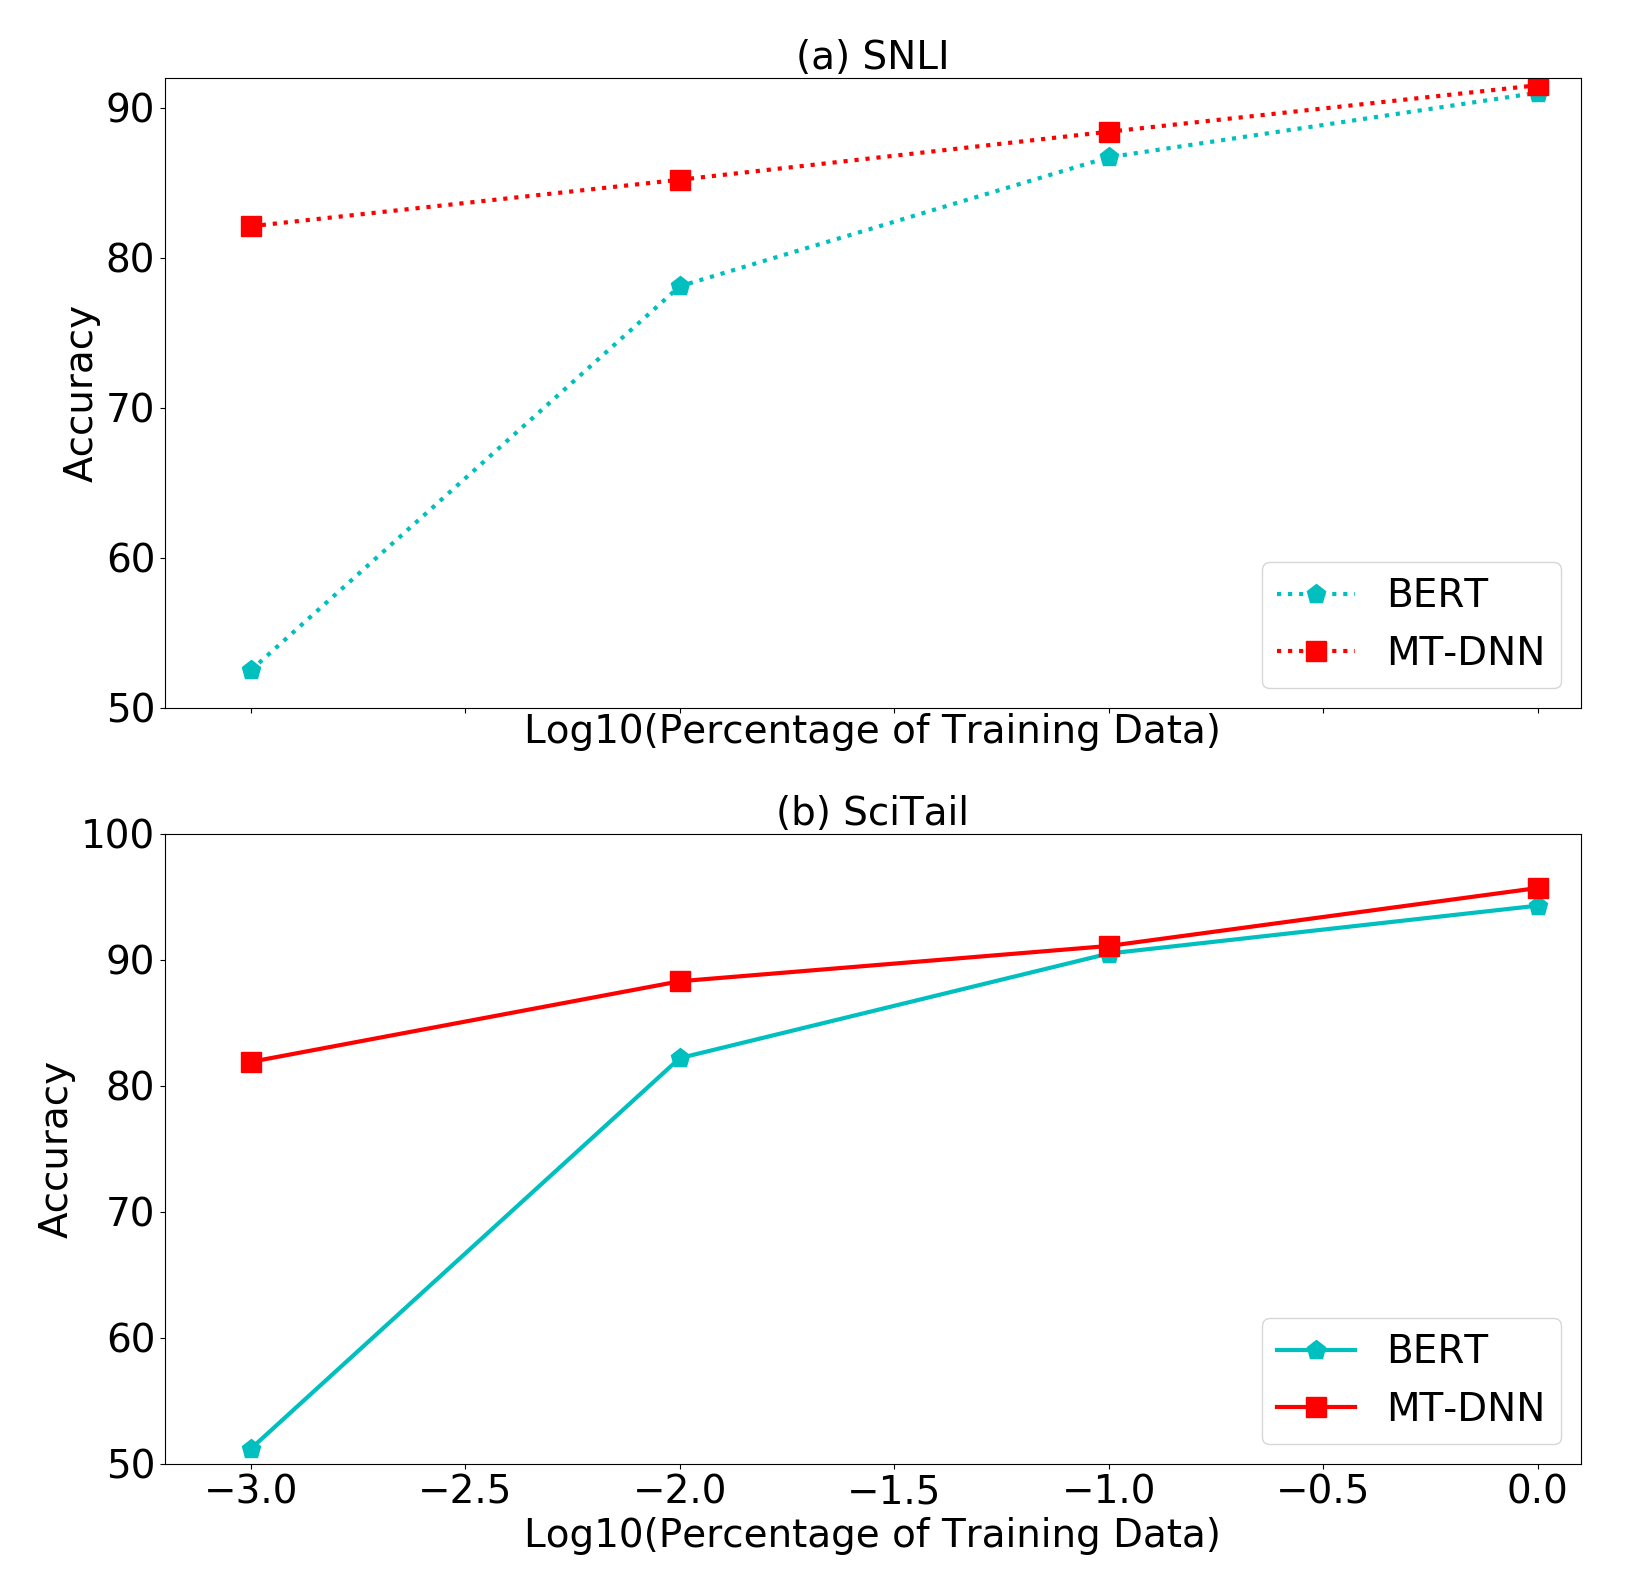
\includegraphics[width=0.48\textwidth]{fig/da.png}
    }   %\vspace{-0.2cm} 
    \caption{\label{fig:domain} Domain adaption results on SNLI and SciTail development datasets using the shared embeddings generated by MT-DNN and BERT, respectively. Both MT-DNN and BERT are fine-tuned based on the pre-trained BERT$_\text{BASE}$. The X-axis indicates the amount of domain-specific labeled samples used for adaptation.}
\end{figure}
\begin{table}[htb!]
	\begin{center}
		\begin{tabular}{@{\hskip1pt}l@{\hskip1pt} |@{\hskip1pt} c |@{\hskip1pt} c |@{\hskip1pt} c | c@{\hskip1pt}}
			\hline \bf Model & 0.1\% & 1\% &10\% & 100\% \\ \hline
            \multicolumn{5}{c}{ SNLI Dataset (Dev Accuracy\%)} \\ \hline
            \#Training Data &549& 5,493& 54,936&549,367 \\ \hline
            BERT &52.5&78.1&86.7 & 91.0 \\ \hline
            MT-DNN &82.1 & 85.2 & 88.4 & 91.5 \\ \hline \hline
\multicolumn{5}{c}{ SciTail Dataset (Dev Accuracy\%)} \\ \hline
            \#Training Data &23& 235& 2,359& 23,596\\ \hline
            BERT &51.2&82.2&90.5 & 94.3 \\ \hline
            MT-DNN &81.9 & 88.3 & 91.1 & 95.7 \\ \hline			
		\end{tabular}
	\end{center}
	\caption{Domain adaptation results on SNLI and SciTail, as shown in Figure~\ref{fig:domain}.  
	}
	\label{tab:domain}
%\lgspace
\end{table}

One of the most important criteria of building practical systems is fast adaptation to new tasks and domains. This is because it is prohibitively expensive to collect labeled training data for new domains or tasks. Very often, we only have very small training data or even no training data.

To evaluate the models using the above criterion, we perform domain adaptation experiments on two NLI tasks, SNLI and SciTail, using the following procedure:
\begin{enumerate}
    \item use the MT-DNN model or the BERT as initial model including both \textit{BASE} and \textit{LARGE} model settings;
    \item create for each new task (SNLI or SciTail) a task-specific model, by adapting the trained MT-DNN using task-specific training data;
    \item evaluate the models using task-specific test data.
\end{enumerate}


We starts with the default training/dev/test set of these tasks. But we randomly sample 0.1\%, 1\%, 10\% and 100\% of its training data. As a result, we obtain four sets of training data for SciTail, which respectively includes  23, 235, 2.3k and 23.5k training samples. Similarly, we obtain four sets of training data for SNLI, which respectively include 549, 5.5k, 54.9k and 549.3k training samples.

We perform  random sampling five times and report the mean among all the runs. Results on different amounts of training data from SNLI and SciTail are reported in Figure~\ref{fig:domain}. We observe that MT-DNN  outperforms the BERT baseline consistently with more details provided in Table \ref{tab:domain}. 
The fewer training examples used, the larger improvement MT-DNN demonstrates over BERT. For example, with only 0.1\% (23 samples) of the SNLI training data, MT-DNN achieves 82.1\% in accuracy while BERT's accuracy is 52.5\%; with 1\%\ of the training data, the accuracy from MT-DNN is 85.2\% and BERT is 78.1\%. We observe similar results on SciTail. 
The results indicate that the representations learned by MT-DNN are more consistently effective for domain adaptation than BERT.


In Table~\ref{tab:nli}, we compare our adapted models, using all in-domain training samples, against several strong baselines including the best results reported in the leaderboards. We see that MT-DNN\textsubscript{LARGE} generates new state-of-the-art results on both datasets, pushing the benchmarks to 91.6\% on SNLI (1.5\% absolute improvement) and 95.0\% on SciTail (6.7\% absolute improvement), respectively. This results in the new state-of-the-art for both SNLI and SciTail. All of these demonstrate the exceptional performance of MT-DNN on domain adaptation.
\begin{table}[htb!]
	\begin{center}
		\begin{tabular}{l | c | c }\hline
	   \bf Model &Dev& Test  \\ \hline 

		\multicolumn{3}{c}{ SNLI Dataset (Accuracy\%)}  \\ \hline 
		GPT \cite{gpt2018} &- & 89.9 \\
		\hline
		\citet{kim2018semantic}$^*$ &- &90.1 \\ \hline 
		BERT\textsubscript{BASE} &91.0 & 90.8 \\
		\hline		
		MT-DNN\textsubscript{BASE} &91.5 & 91.1 \\
		\hline
		BERT\textsubscript{LARGE} &91.7& 91.0\\ \hline		
		{\MNAME}\textsubscript{LARGE}&\textbf{92.2}& \textbf{91.6}\\ \hline		
		\hline
		\multicolumn{3}{c}{ SciTail Dataset (Accuracy\%)}  \\ \hline 	GPT \cite{gpt2018}$^*$ &- &88.3 \\ \hline
		BERT\textsubscript{BASE} &94.3 & 92.0 \\ \hline
		MT-DNN\textsubscript{BASE} &95.7 &94.1 \\
		\hline
		BERT\textsubscript{LARGE} &95.7& 94.4\\ \hline		
		{\MNAME}\textsubscript{LARGE} &\textbf{96.3}& \textbf{95.0}\\ \hline		
		\end{tabular}
	\end{center}
	%\lgspace
	 %\vspace{-0.3cm}
	\caption{Results on the SNLI and SciTail dataset. Previous state-of-the-art results are marked by $*$, obtained from the official SNLI leaderboard (https://nlp.stanford.edu/projects/snli/) and the official SciTail leaderboard maintained by AI2 (https://leaderboard.allenai.org/scitail). 
	%Both MT-DNN and BERT are fine-tuned based on the pre-trained BERT$_\text{BASE}$.
	}
	\label{tab:nli}
%\lgspace

\end{table}


